%
% Copyright (C) 2011 Agostino De Marco
%                    <agostino dot demarco at unina dot it>
%                    Roberto Giacomelli
%                    <giaconet dot mailbox at gmail dot com>
%
%    This work may be distributed and/or modified under the
%    conditions of the LaTeX Project Public License, either
%    version 1.3 of this license or any later version.
%    The latest version of this license is in
%    http://www.latex-project.org/lppl.txt and version 1.3
%    or later is part of all distributions of LaTeX version
%    2005/12/01 or later.
%
% This work has the LPPL maintenance status `maintained'.
% 
% The Current Maintainer of this work are Agostino De Marco
% and Roberto Giacomelli
%
\documentclass{standalone}
\usepackage{lmodern}
\usepackage{amsmath,fixmath}
\usepackage{relsize}
\usepackage{pgfplots}
\usepackage{siunitx}

\pgfplotsset{compat=1.3}

\addtolength{\oddsidemargin}{0cm}

\begin{document}

\pgfkeys{
   /pgf/number format/.cd,
      use comma
}
\pgfplotsset{
   every axis/.append style={
      font=\relsize{2},
      % very thick,% thick
      % tick style={very thick} % semithick
      line width=1.2pt,% thick
      tick style={line width=1.2pt} % semithick
      },
   major grid style={
      line width = 0.6pt,
      gray,
      dash pattern=on 16pt off 4pt
   },
   every axis title/.append style={
      font=\relsize{3}
   }
}

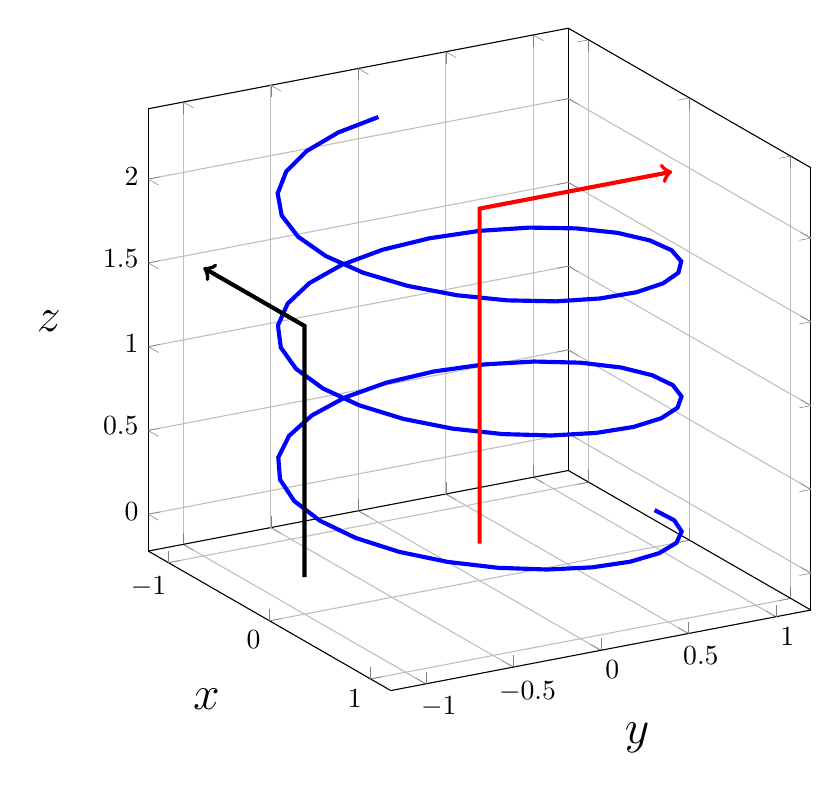
\begin{tikzpicture}
\begin{axis}[
   width=10cm, height=10cm,
   view={60}{20},
   xmin=-1.2, xmax=1.2,
   ymin=-1.2, ymax=1.2,
   grid = major,
   xlabel=$x$, ylabel=$y$, zlabel=$z$,
   every axis x label/.style={
      at={(rel axis cs:0.5,-0.15,-0.15)},font=\relsize{3}},
   every axis y label/.style={
      at={(rel axis cs:1.15,0.5,-0.15)},font=\relsize{3}},
   every axis z label/.style={
      at={(rel axis cs:-0.15,-0.15,0.5)},font=\relsize{3}},
   variable=\t
   ]

\addplot3+[domain=0:5.5*pi,samples=70,samples y=0,no marks,line width=1.5pt]
   ({sin(deg(t))}, {cos(deg(t))}, {2*t/(5*pi)});

\addplot3 +[->,no marks,line width=1.5pt]
   coordinates {(0,0,0) (0,0,2) (0,1.1,2)};

\draw[->,line width=1.5pt] (axis cs:0,-1,0) -- (axis cs:0,-1,1.5) -- (axis cs:-1,-1,1.5);

\end{axis}
\end{tikzpicture}

\end{document}